\chapter{字符串管理}

任何程序都需要管理字符串。管理就像分配、搜索、连接、扩展、收缩等等。

字符串需要许多操作。 尽管C标准库为这一目标提供了许多功能,但C经典字符串,即\code{char *}(或\code{char []})在PHP这样的强程序中按原样使用通常有点弱。

因此,PHP在C字符串之上设计了一个层:\keyword{zend\_strings}。另外还存在另一个API,它实现了C经典字符串或\keyword{zend\_strings}常见的字符串操作: \keyword{smart\_str} API。

\section{字符串管理:zend\_string}
\label{sec:zend_string}

它增加了内存管理功能,以便相同字符串可以在多个地方共享,而不需要复制它。另外一些字符串被“扣押”,即它们被“持久”分配并由内存管理器专门管理,因此它们不会在多个请求中被销毁。 这些内存稍后将从\href{http://www.phpinternalsbook.com/php7/memory_management/zend_memory_manager.html}{Zend内存管理器}获得永久分配。

\subsection{结构和访问宏}

下面是\keyword{zend\_string}结构:

\begin{lstlisting}[language=c]
struct _zend_string {
        zend_refcounted_h gc;           /*gc信息*/
        zend_ulong        h;            /* hash value */
        size_t            len;          /*字符串长度*/
        char              val[1];       /*字符串起始地址*/
};
\end{lstlisting}

如您所见,该结构嵌入了\code{zend\_refcounted\_h}头。这样做是为了内存管理和引用。由于字符串很可能用作哈希表查询的键,所以它将其哈希值嵌入到\keyword{h}字段中。这是一个无符号long \code{zend\_ulong}。
此数字仅在需要对\code{zend\_string}进行哈希处理时使用,尤其是与\href{http://www.phpinternalsbook.com/php7/internal_types/hashtables.html}{HashTables zend\_array}一起使用时; 这很可能。


如您所知,可以通过\keyword{len}字段知道字符串的长度,用来支持“二进制字符串”。二进制字符串是嵌入一个或多个\keyword{NUL}字符(\textbackslash{}0)的字符串。当传递给libc函数时,这些字符串将被截断,否则它们的长度将无法正确计算。所以在\keyword{zend\_string}中,字符串的长度总是已知的。请注意,计算ASCII字符(字节)数量的长度,不计算结尾的\keyword{NUL},但是计算可能在中间的NULs。例如,字符串“foo”在\keyword{zend\_string}中存储为“foo\textbackslash{}0”,其长度为3。此外,字符串“foo\textbackslash{}0bar”将存储为“foo\textbackslash{}0bar\textbackslash{}0”,长度将为7。

最后,字符存储在\code{char [1]}字段中。这不是一个\code{char *},而是一个\code{char[1]}。为什么?这是一种名为“C struct hack”的内存优化。(你可以搜索一下这些术语)。基本上,它允许引擎为\code{zend\_string}结构和要存储的字符分配空间,作为一个单独的C指针。这优化了内存访问,因为内存将是一个连续分配的块,而不是内存中稀疏的两个块
(一个用于\code{zend\_string *},一个用于存储到其中的\code{char *})。

struct hack一定要记住,因为内存布局看起来像C字符位于C \code{zend\_string}结构的末尾,在使用C调试器(或在调试字符串时)时可能会感觉到/看到。这个hack完全由你在操作\code{zend\_string}结构时使用的API管理。

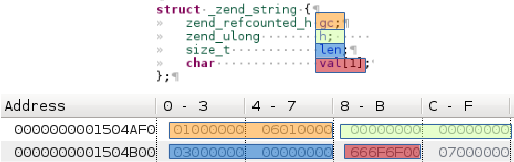
\includegraphics{images/zend_string_memory_layout.png} 

\subsection{使用\code{zend\_string} API}

\subsubsection{简单实例}

与\keyword{Zvals}一样,您不要手工操作\code{zend\_string}内部字段,而是始终要使用宏。还有一些宏可以触发字符串上的操作。这些不是函数,而是宏,都存储在所需的\href{https://github.com/php/php-src/blob/PHP-7.0/Zend/zend_string.h}{Zend/zend\_string.h}头:

\begin{lstlisting}[language=c]
zend_string *str;

str = zend_string_init("foo", strlen("foo"), 0);
php_printf("This is my string: %s\n", ZSTR_VAL(str));
php_printf("It is %zd char long\n", ZSTR_LEN(str));

zend_string_release(str);
\end{lstlisting}

上面的简单示例展示了基本的字符串管理。

\code{zend\_string\_init()}函数(它实际上是宏,但是让我们传入这些细节)应当传入完整\code{char *}型C字符串及其长度。最后一个参数(类型为int)值应该是0或1。如果传0,则要求引擎使用Zend内存管理器使用请求绑定堆分配。这种分配将在当前请求结束时销毁。如果您不这样做,在调试构建时,引擎将会对您刚刚创建的发出内存泄漏的警告。如果传1,您将请求我们所说的“持久”分配,即引擎将调用传统的C \code{malloc()}方法,并且不会以任何方式跟踪内存分配。

\alertinfo{如果您想了解有关内存管理的更多信息,可以阅读\href{http://www.phpinternalsbook.com/php7/memory_management.html}{专门章节}。}

然后,我们输出字符串。 我们使用\code{ZSTR\_VAL()}宏访问字符数组。\code{ZSTR\_LEN()}获取长度信息。 \code{zend\_string}相关的宏都以\code{ZSTR\_**()}开头,请注意这与\code{Z\_STR**()}宏不同。

\alertinfo{长度使用\code{size\_t}类型存储。因此为了输出它\code{printf()}需要使用"\%zd"。您应该始终使用正确的\code{printf()}格式。如果不这样做可能会导致应用程序崩溃或产生安全问题。有关printf()格式的精彩回忆,请访问\href{http://www.cplusplus.com/reference/cstdio/printf/}{此链接}}

最后,我们使用\code{zend\_string\_release()}释放字符串。这个"释放"是强制性的。这是关于内存管理的。“释放”是一个简单的操作:减少字符串的引用计数器,如果它变为0,API将为你释放字符串。如果忘记释放字符串,很可能会造成内存泄漏。

\alertinfo{您必须始终考虑C语言中的内存管理。如果您分配内存-无论是直接使用\code{malloc()},还是使用API来完成,你必须在某个时刻进行\code{free()}。如果不这样做会造成内存泄露并会变成没有人能够安全使用的设计糟糕的程序}

\subsubsection{使用hash}

如果需要访问hash值,请使用\code{ZSTR\_H()}。但是,创建\code{zend\_string}时不会自动计算哈希值。但是当使用HashTable API操作字符串时,它将会完成计算。如果你想强制立即计算hash值,可以使用\code{ZSTR\_HASH()}或者\code{zend\_string\_hash\_val()}。一旦计算出hash值,它将会被保存并且不会再次被计算。如果处于某种原因,您需要重新计算它 - 例如:因为你更改了字符串的值 - 使用\code{zend\_string\_forget\_hash\_val()}:



\begin{lstlisting}[language=c]
        zend_string *str;

        str = zend_string_init("foo", strlen("foo"), 0);
        php_printf("This is my string: %s\n", ZSTR_VAL(str));
        php_printf("It is %zd char long\n", ZSTR_LEN(str));
        
        zend_string_hash_val(str);
        php_printf("The string hash is %lu\n", ZSTR_H(str));
        
        zend_string_forget_hash_val(str);
        php_printf("The string hash is now cleared back to 0!");
        
        zend_string_release(str);
\end{lstlisting}


\subsubsection{字符串复制及内存管理}

\code{zend\_string} API的一个非常好的特性是它允许一部分通过简单地声明对它的兴趣来“拥有”一个字符串。 然后引擎不会在内存中复制字符串,而只是递增其引用计数(作为其\code{zend\_refcounted\_h}的一部分)。这就在代码中实现了内存共享。

那样的话,当我们说“复制”(copying)\code{zend\_string}时,事实上,我们不会在内存中复制任何东西。如果需要 - 这仍然是一个可能的操作 - 我们然后讨论“复制”(duplicating)字符串。 我们开始吧:

\begin{lstlisting}[language=c]

        zend_string *foo, *bar, *bar2, *baz;

        foo = zend_string_init("foo", strlen("foo"), 0); /* creates the "foo" string in foo */
        bar = zend_string_init("bar", strlen("bar"), 0); /* creates the "bar" string in bar */

        /* creates bar2 and shares the "bar" string from bar into bar2. Also increments the refcount of the "bar" string to 2 */
        bar2 = zend_string_copy(bar);

        php_printf("We just copied two strings\n");
        php_printf("See : bar content : %s, bar2 content : %s\n", ZSTR_VAL(bar), ZSTR_VAL(bar2));

        /* Duplicate in memory the "bar" string, create the baz variable and make it solo owner of the newly created "bar" string */
        baz = zend_string_dup(bar, 0);

        php_printf("We just duplicated 'bar' in 'baz'\n");
        php_printf("Now we are free to change 'baz' without fearing to change 'bar'\n");

        /* Change the last char of the second "bar" string turning it to "baz" */
        ZSTR_VAL(baz)[ZSTR_LEN(baz) - 1] = 'z';

        /* Forget the old hash (if computed) as now the string changed, thus its hash must also change and get recomputed */
        zend_string_forget_hash_val(baz);

        php_printf("'baz' content is now %s\n", ZSTR_VAL(baz));

        zend_string_release(foo);  /* destroys (frees) the "foo" string */
        zend_string_release(bar);  /* decrements the refcount of the "bar" string to one */
        zend_string_release(bar2); /* destroys (frees) the "bar" string both in bar and bar2 vars */
        zend_string_release(baz);  /* destroys (frees) the "baz" string */
        
\end{lstlisting}    

我从分配"foo"和"bar“开始。然后我们创建了作为\code{bar}副本的\code{bar2}字符串。在这里,我们要知道:\code{bar}和\code{bar2}在内存中指向相同的C字符串,修改其中一个字符串就会改变第二个。这就是\code{zend\_string\_copy()}的行为:它只增加所拥有的C字符串的refcount值。

如果我们想分开这两个字符串 - 即我们希望那个字符串在内存中有两个不同的副本 - 我们需要使用\code{zend\_string\_dup()}复制。然后我们将bar2变量的字符串复制到baz变量中。现在,baz变量嵌入了自己的字符串副本,并且可以在不影响bar2的情况下更改它。这就是我们所做的:我们将bar中的最后一个r用z替换为baz。然后我们打印他们,并释放每个字符串的内存。

请注意我们忘记了hash值(我们如果之前计算过它,则无需考虑该细节)。这是一个值得记住的好习惯。如前所述,如果\code{zend\_string}被用做HashTables的一部分,hash则被使用了。这在开发中是非常常见的操作,更改字符串值也需要重新计算hash值。忘记这一步将导致可能花费一些时间来跟踪的bug。

\subsubsection{字符串操作}

\code{zend\_string} API允许其他操作,例如扩展或缩小字符串,更改其大小写或比较。目前还没有可用的联合操作,但这很容易执行:

\begin{lstlisting}[language=c]
        zend_string *FOO, *bar, *foobar, *foo_lc;

        FOO = zend_string_init("FOO", strlen("FOO"), 0);
        bar = zend_string_init("bar", strlen("bar"), 0);
        
        /* Compares a zend_string against a C string literal */
        if (!zend_string_equals_literal(FOO, "foobar")) {
            foobar = zend_string_copy(FOO);
        
            /* reallocates the C string to a larger buffer */
            foobar = zend_string_extend(foobar, strlen("foobar"), 0);
        
            /* concatenates "bar" after the newly reallocated large enough "FOO" */
            memcpy(ZSTR_VAL(foobar) + ZSTR_LEN(FOO), ZSTR_VAL(bar), ZSTR_LEN(bar));
        }
        
        php_printf("This is my new string: %s\n", ZSTR_VAL(foobar));
        
        /* Compares two zend_string together */
        if (!zend_string_equals(FOO, foobar)) {
            /* duplicates a string and lowers it */
            foo_lc = zend_string_tolower(foo);
        }
        
        php_printf("This is FOO in lower-case: %s\n", ZSTR_VAL(foo_lc));
        
        /* frees memory */
        zend_string_release(FOO);
        zend_string_release(bar);
        zend_string_release(foobar);
        zend_string_release(foo_lc);
\end{lstlisting}  

\subsubsection{使用zvals访问zend\_string}

既然您已经知道如何管理和操作\code{zend\_string},那么让我们看看它们与zval容器之间的交互。

注意:
你需要熟悉zvals,如果不熟悉,请阅读:zvals一章。
这些宏允许您将\code{zend\_string}存储到zval中,或者从zval读取\code{zend\_string}:

\begin{lstlisting}[language=c]
        zval myval;
        zend_string *hello, *world;

        zend_string_init(hello, "hello", strlen("hello"), 0);

        /* Stores the string into the zval */
        ZVAL_STR(&myval, hello);

        /* Reads the C string, from the zend_string from the zval */
        php_printf("The string is %s", Z_STRVAL(myval));

        zend_string_init(world, "world", strlen("world"), 0);

        /* Changes the zend_string into myval : replaces it by another one */
        Z_STR(myval) = world;

/* ... */
\end{lstlisting} 

您必须记住的是,以\code{ZSTR\_***(s)}开头的每个宏都将作用于\code{zend\_string}。

\begin{itemize}
    \item ZSTR\_VAL()
    \item ZSTR\_LEN()
    \item ZSTR\_HASH()
    \item ...
\end{itemize}

以\code{Z\_STR**(z)}开头的每个宏都将作用于嵌入到zval中的\code{zend\_string}

\begin{itemize}
        \item Z\_STRVAL()
        \item Z\_STRLEN()
        \item Z\_STRHASH()
        \item ...
\end{itemize}

其他存在的一些你可能用不到。

\subsubsection{PHP的历史和经典的C字符串}

简单介绍一下经典的C字符串。在C语言中,字符串是字符数组(char foo[])或者是指向字符的指针(char *)。他们对自己的长度一无所知,这就是以NUL终止的原因(知道字符串的开始和结束,你就知道了它的长度)。

在PHP 7之前,\code{zend\_string}结构根本不存在。老版本使用了传统的char * / int 对。 你仍然可以在PHP源代码中找到很少的地方,还在使用char */ int 对而不是\code{zend\_string}。 你还可以找到API工具,在\code{zend\_string}和char * / int 对之间进行交互。

尽可能:使用\code{zend\_string}。 一些罕见的地方没有使用\code{zend\_string},因为在那个地方使用它们是无关紧要的,但是你会在PHP源代码中找很多对\code{zend\_string}的引用。

\subsubsection{Interned zend\_string}

在这里简单介绍一下interned字符串。在扩展开发中,您应该很少会需要这样的概念。Interned字符串还与OPCache扩展有交互。

Interned字符串是重复数据删除的字符串. 当使用OPCache时,它们从一个请求到另一个请求还会被重复使用。

假设您要创建字符串“foo”。 你倾向于做的只是创建一个新的字符串“foo”:

\begin{lstlisting}[language=c]
zend_string *foo;
foo = zend_string_init("foo", strlen("foo"), 0);

/* ... */
\end{lstlisting} 

但是问题来了:那部分字符串是不是在你使用之前就已经创建完成?当您需要一个字符串时,你的代码会在PHP生命中的某个时刻执行,这意味着在您之前发生的一些代码可能需要完全相同的字符串(以“foo”为例)。

interned字符串是关于要求引擎探测interned字符串储存区,如果它可以找到你的字符串,就可以重用已分配的指针。如果不存在:创建一个新的字符串并且“intern”它,这使得它可以用于PHP源代码的其他部分(其他扩展、引擎本身等等)。


下面是一个例子:

\begin{lstlisting}[language=c]

        zend_string *foo;
        foo = zend_string_init("foo", strlen("foo"), 0);

        foo = zend_new_interned_string(foo);

        php_printf("This string is interned : %s", ZSTR_VAL(foo));

        zend_string_release(foo);
        
\end{lstlisting}


在上面的代码中,我们创建了一个非常经典的\code{zend\_string}。然后,我们将创建的\code{zend\_string}传递给\code{zend\_new\_interned\_string()}。这个函数在引擎内的interned字符串缓冲区中寻找相同的字符串(这里是“foo”)。如果找到了它(意味着有人已经创建了这个字符串),那么它将释放您的字符串(可能释放它),并将用来自interned字符串缓冲区的字符串替换它。如果没有查到它:会将它添加到interned字符串缓冲区中,因此可供将来使用或PHP的其他部分使用。

你必须注意内存分配。interned字符总是将refcount设置为1,因为他们不需要被计数,因为它们将与interned字符串缓冲区共享,因此不能被销毁。

例:

\begin{lstlisting}[language=c]

        zend_string *foo, *foo2;

        foo  = zend_string_init("foo", strlen("foo"), 0);
        foo2 = zend_string_copy(foo); /* increments refcount of foo */

        /* refcount falls back to 1, even if the string is now
        * used at three different places */
        foo = zend_new_interned_string(foo);

        /* This doesn't do anything, as foo is interned */
        zend_string_release(foo);

        /* This doesn't do anything, as foo2 is interned */
        zend_string_release(foo2);

        /* At the end of the process, PHP will purge its interned
        string buffer, and thus free() our "foo" string itself */
\end{lstlisting}

这都是关于垃圾回收的。

当一个字符串是interned时,它的GC标志通过添加\code{IS\_STR\_INTERNED}标志来改变,无论他们使用什么内存分配类(永久的或基于请求的)。当你想复制或者释放一个字符串时会查询这个标志。如果这个字符串是interned,引擎在复制字符串时不会增加它的refcount。但是如果你释放(release)字符串时,它也不会减少或者释放(free)它。它什么也不会做。在进程生命周期结束时,它将销毁其interned字符串缓冲区,并释放interned字符串。

实际上,如果OPCache启动,这个过程会比这个要复杂一点。OPCache扩展改变了interned字符串的使用方式。在没有OPCache的情况下,如果您在请求的过程中创建了一个interned \code{zend\_string},那么该字符串将在当前请求的末尾被清除,并且不会被下一次请求重用。但是,如果您使用OPCache,那么interned字符串将存储在一个共享内存段中,并在同一个池中的每个PHP进程之间共享。此外,interned字符串会跨多个请求重用。

interned字符串可以节省内存,因为相同的字符串在内存中存储的次数不会超过一次。当时它可能会耗一些CPU时间,因为它经常需要查找interned字符串存储,即使该进程已经过优化。作为扩展开发者,以下是全局规则:

\begin{itemize}
        \item 如果使用OPCache(应该是这样),并且如果您需要创建请求绑定的只读字符串:使用interned字符串
        \item 如果您需要一个字符串,您确信知道PHP已经interned的字符串(一个众所周知的PHP字符串,例如“php”或者“str\_replace”),请使用一个interned字符串
        \item 如果字符串不是只读的,并且在创建字符串后可以/应该进行更改,则不要使用interned字符串
        \item 如果将来不太可能重用该字符串,则不要使用interned字符串
\end{itemize}

Interned字符串的详细介绍在\href{https://github.com/php/php-src/blob/PHP-7.0/Zend/zend_string.c}{Zend/zend\_string.c}


\section{smart\_str API}

这看起来可能很奇怪,C语言几乎没有提供任何字符串处理功能(构建、连接、收缩、展开、转换等等)。C是一种低级通用语言,可用于构建API以处理更具体的任务,例如字符串构造。

\alertinfo{显然,你们都知道我们讨论的是ASCII字符串,也就是字节。而不是Unicode。}

PHP的`smart\_str` API 可以帮助你构建字符串特别是将字节块连接为字符串。这些API位于:\href{http://www.phpinternalsbook.com/php7/internal_types/strings/printing_functions.html}{PHP’s special printf() APIs} 和\href{http://www.phpinternalsbook.com/php7/internal_types/strings/zend_strings.html}{zend\_string} 用来帮助字符串管理。

\subsection{smart\_str VS smart\_string}

下面是两种结构体:

\begin{lstlisting}[language=c]

    typedef struct {
        char *c;
        size_t len;
        size_t a;
    } smart_string;

    typedef struct {
        zend_string *s;
        size_t a;
    } smart_str;

\end{lstlisting}


如您所见,一个将使用传统的C字符串(如\code{char*/size\_t}),另一个将使用PHP的特定\code{zend\_string}结构。

我们将详细说明后者:\code{smart\_str},它与\href{http://www.phpinternalsbook.com/php7/internal_types/strings/zend_strings.html}{zend\_strings}一起使用。这两个API完全相同,只需注意一个(我们将在这里详述的那个)由\code{smart\_str\_**()}开头,另一个由\code{smart\_string\_***()}开头。不要混淆!

\code{smart\_str} API详细介绍在\href{https://github.com/php/php-src/blob/509f5097ab0b578adc311c720afcea8de266aadd/Zend/zend_smart_str.h}{Zend/zend\_smart\_str.h}(也是 .c 文件)。

\alertwarning{不要将\code{smart\_str}与\code{smart\_string}混淆。}

\subsection{基本API使用}

到目前为止,这个API非常容易管理。

您在堆栈分配一个\code{smart\_str},并将其指针传递给\code{smart\_str\_***()}API函数,它为您管理内含的\code{zend\_string}。 你构建你的字符串,使用它,然后释放它。里面没什么强大的东西,对吗?

内含的\code{zend\_string}将要\href{http://www.phpinternalsbook.com/php7/memory_management/zend_memory_manager.html}{被永久的或者请求绑定}的分配,这取决于您将使用的最后一个扩展API参数:

\begin{lstlisting}[language=c]
        smart_str my_str = {0};

        smart_str_appends(&my_str, "Hello, you are using PHP version ");
        smart_str_appends(&my_str, PHP_VERSION);

        smart_str_appendc(&my_str, '\n');

        smart_str_appends(&my_str, "You are using ");
        smart_str_append_unsigned(&my_str, zend_hash_num_elements(CG(function_table)));
        smart_str_appends(&my_str, " PHP functions");

        smart_str_0(&my_str);

        /* Use my_str now */
        PHPWRITE(ZSTR_VAL(my_str.s), ZSTR_LEN(my_str.s));

        /* Don't forget to release/free it */
        smart_str_free(&my_str);

\end{lstlisting}  


我们在这里使用了简单的API,扩展以\code{\_ex()}为结尾,允许你选择\keyword{zend\_string}是持久或者是请求绑定时分配。例如:

\begin{lstlisting}[language=c]
        smart_str my_str = {0};

        smart_str_appends_ex(&my_str, "Hello world", 1); /* 1 means persistent allocation */
\end{lstlisting} 

然后,根据你想要追加的内容,你需要调用正确的API。如果你追加一个经典的C字符串,你可以使用\code{smart\_str\_appends(smart\_str *dst, const char *src)}。如果你追加二进制字符串并且知道它的长度,你可以使用\code{smart\_str\_appendl(smart\_str *dst, const char *src, size\_t len)}。

\code{smart\_str\_append(smart\_str *dest, const zend\_string *src)}只是讲\code{zend\_string} 追加到\code{smart\_str}。如果你想追加其他的\code{smart\_str},使用\code{smart\_str\_append\_smart\_str(smart\_str *dst, const smart\_str *src)}来合并它们。

\subsection{smart\_str特定技巧}

\begin{itemize}
        \item 永远不要忘记通过调用\code{smart\_str\_0()}来完成你的字符串。此操作会在内含的字符串末尾追加一个NUL字符,会使其用libc字符串函数兼容
        \item 永远不要忘记在使用完成字符串后通过\code{smart\_str\_free()}来释放(free)。
        \item \code{smart\_str}内含一个\code{zend\_string},允许你通过使用其reference计数在后面的其他地方共享它。请访问\href{http://www.phpinternalsbook.com/php7/internal_types/strings/zend_strings.html}{zend\_string专用章节}了解更多信息。
        \item 你可以考虑一下\code{smart\_str}分配。了解一下\code{smart\_str\_alloc()} 系列。
        \item \code{smart\_str}被大量的用于PHP的核心代码。例如:PHP的特定函数\href{http://www.phpinternalsbook.com/php7/internal_types/strings/printing_functions.html}{printf()}在内部使用了\code{smart\_str}缓冲区。
        \item \code{smart\_str}绝对是一个您需要掌握的简单结构。
\end{itemize}  


\section{PHP自定义的printf函数}








































